%%%%%%%%%%%%%%%%%%%%%%%%%%%%%%%%%%%%%%%%%%%%%%%%%%%%%%%%%%%%
%%%  Augmenting TV Newscasts via Entity Expansion  %%%
%%%%%%%%%%%%%%%%%%%%%%%%%%%%%%%%%%%%%%%%%%%%%%%%%%%%%%%%%%%%

\documentclass{llncs}

\newcommand{\superscript}[1]{\ensuremath{^{\textrm{#1}}}}

\usepackage{makeidx}  % allows for indexgeneration
\usepackage[hyphens]{url}
\usepackage{textcomp}
\usepackage{color}
\usepackage{listings}
\usepackage{multirow}
\usepackage{mathtools}
\usepackage{graphicx}
\usepackage{fancyvrb}
\usepackage{amsmath}
\usepackage{graphicx}
\usepackage[font=small,labelfont=bf]{caption}
\setcounter{MaxMatrixCols}{20}
\usepackage{pbox}
\usepackage{amsfonts}


% listing styles
\lstset{numbers=left, numberstyle=\tiny,basicstyle=\ttfamily\scriptsize, tabsize=2, keywordstyle=\underbar, stringstyle=\small, backgroundcolor=\color[gray]{0.94}, framexleftmargin=2pt}
\lstdefinestyle{rdfa}{numberblanklines=true, morekeywords={}}



\begin{document}
\frontmatter          % for the preliminaries
\pagestyle{headings}  % switches on printing of running heads
\mainmatter              % start of the contributions

\title{Augmenting TV Newscasts via Entity Expansion}
\author{Jos\'e Luis Redondo Garc\'ia\inst{2}, Michiel Hildebrand\inst{1}, Lilia Perez Romero\inst{1}, Rapha\"el Troncy\inst{2}}
\institute{CWI, Amsterdam, The Netherlands, \\
\email{\{M.Hildebrand, L.Perez\}@cwi.nl}
\and
EURECOM, Sophia Antipolis, France, \\
\email{\{redondo, raphael.troncy\}@eurecom.fr}
}


\maketitle              % typeset the title of the contribution

%%%%%%%%%%%%%%%%%%
%%%  Abstract  %%%
%%%%%%%%%%%%%%%%%%

\begin{abstract}
We present an approach that leverages on the knowledge present on the Web for identifying and enriching relevant items inside a News video and displaying them in a timely and user friendly fashion. 
This second screen prototype (i) collects and offers information about persons, locations, organizations and concepts occurring in the newscast, and (ii) combines them for enriching the underlying story along five main dimensions: expert's opinions, timeline, in depth, in other sources, and geo-localized comments from other viewers.  
Starting from preliminary insights coming from the named entities spotted on the video subtitles, we expand this initial context to a broader event representation by relying in the knowledge of other non-structured Web documents talking about the same fact. This makes possible to generate a much richer, context aware metadata of a TV program that boost the viewer interaction and opens new possibilities in the hyperlinked television domain. 

\keywords{Multimedia Annotation, Entity Expansion, Newscast Enrichment}
\end{abstract}

%%%%%%%%%%%%%%%%%%%%%%%%%
%%%  1. Introduction  %%%
%%%%%%%%%%%%%%%%%%%%%%%%%

\section{Introduction}
Second screen applications are a popular approach to enrich the TV viewing experience. Within the LinkedTV project we developed a second screen application for News broadcasts. The functionality and the design of this application is the result of a user-centred design process involving focus groups, interviews, iterative design and evaluation~\cite{Lilia report}. The initial design and evaluation of the prototype was done with manually curated content. This was deliberately chosen, as we did not want the quality of the content impact the evaluation of the design. In practice, the manual curation of the content is, however, not feasible, as it is too time consuming for a broadcaster.

This paper provides a solution to automatically generate the content for the LinkedTV News second screen application. The application supports two modes of interaction. The passive mode gives the user access to factual information about persons, locations and organisations that are related to a news item. Figure 1a shows a screenshot of the passive mode. Per news item the application shows eight entities. Therefore, to generate the content for the passive mode we need a solution that finds the eight most relevant entities to the user. A typical approach is to use Named Entity Recognition (NER) over the textual information attached to particular video fragment, and by linking the entities to real world objects using web identifiers (Named Entity Disambiguation), we also have the content to present to the user. A growing number of APIs provide such a service, like AlchemyAPI\footnote{\fontsize{8pt}{1em}\selectfont \url{http://www.alchemyapi.com/}} or DBpedia Spotlight\footnote{\fontsize{8pt}{1em}\selectfont \url{http://spotlight.dbpedia.org/}}.  If the textual information attached to a video contains temporal references (e.g. subtitles), it is possible to align the entities with the time when they appear in the video. In this line, Yunjia et al.~\cite{yunjia2013} have proved that named entity recognition techniques applied on video subtitles can produce good results for video classification. 
In the manual curation of the content we, however, experienced that relevant entities do not only occur in the subtitles, but can also be related to the video indirectly. Therefore, we propose an extension of entity extraction on the subtitles alone by also looking for entities in Web documents that are related to the video. Our solution uses a selected number of entities from the subtitles to find related Web documents, using a Google custom search engine. From the top ranked documents we extract additional entities and rank the total set of entities to get the top eight for the interface.

The active mode of the LinkedTV news second screen application allows the user to explore  background and related information to a news item. As shown in Figure 1b the application provides 5 browsing dimensions for exploration. Each dimension expects a set of Web documents that fit the dimensions, such as articles about the same news item (or topic), but from various sources, or opinion articles from specific journalists. To find these document we propose the use of a Google custom search engine and a method to generate the queries that is tailored to content requirements of the different dimensions.

In the remainder of this paper we briefly describe the interface of the appliction, explain the algorithms to generate the content for the passive and active mode.

%%%%%%%%%%%%%%%%%%%%%%%%%%
%%%  Augmenting and Enriching TV News    %%%
%%%%%%%%%%%%%%%%%%%%%%%%%%

\section{LinkedTV News companion application}
\label{sec:tvnews}

\begin{figure}[h!]
\centering
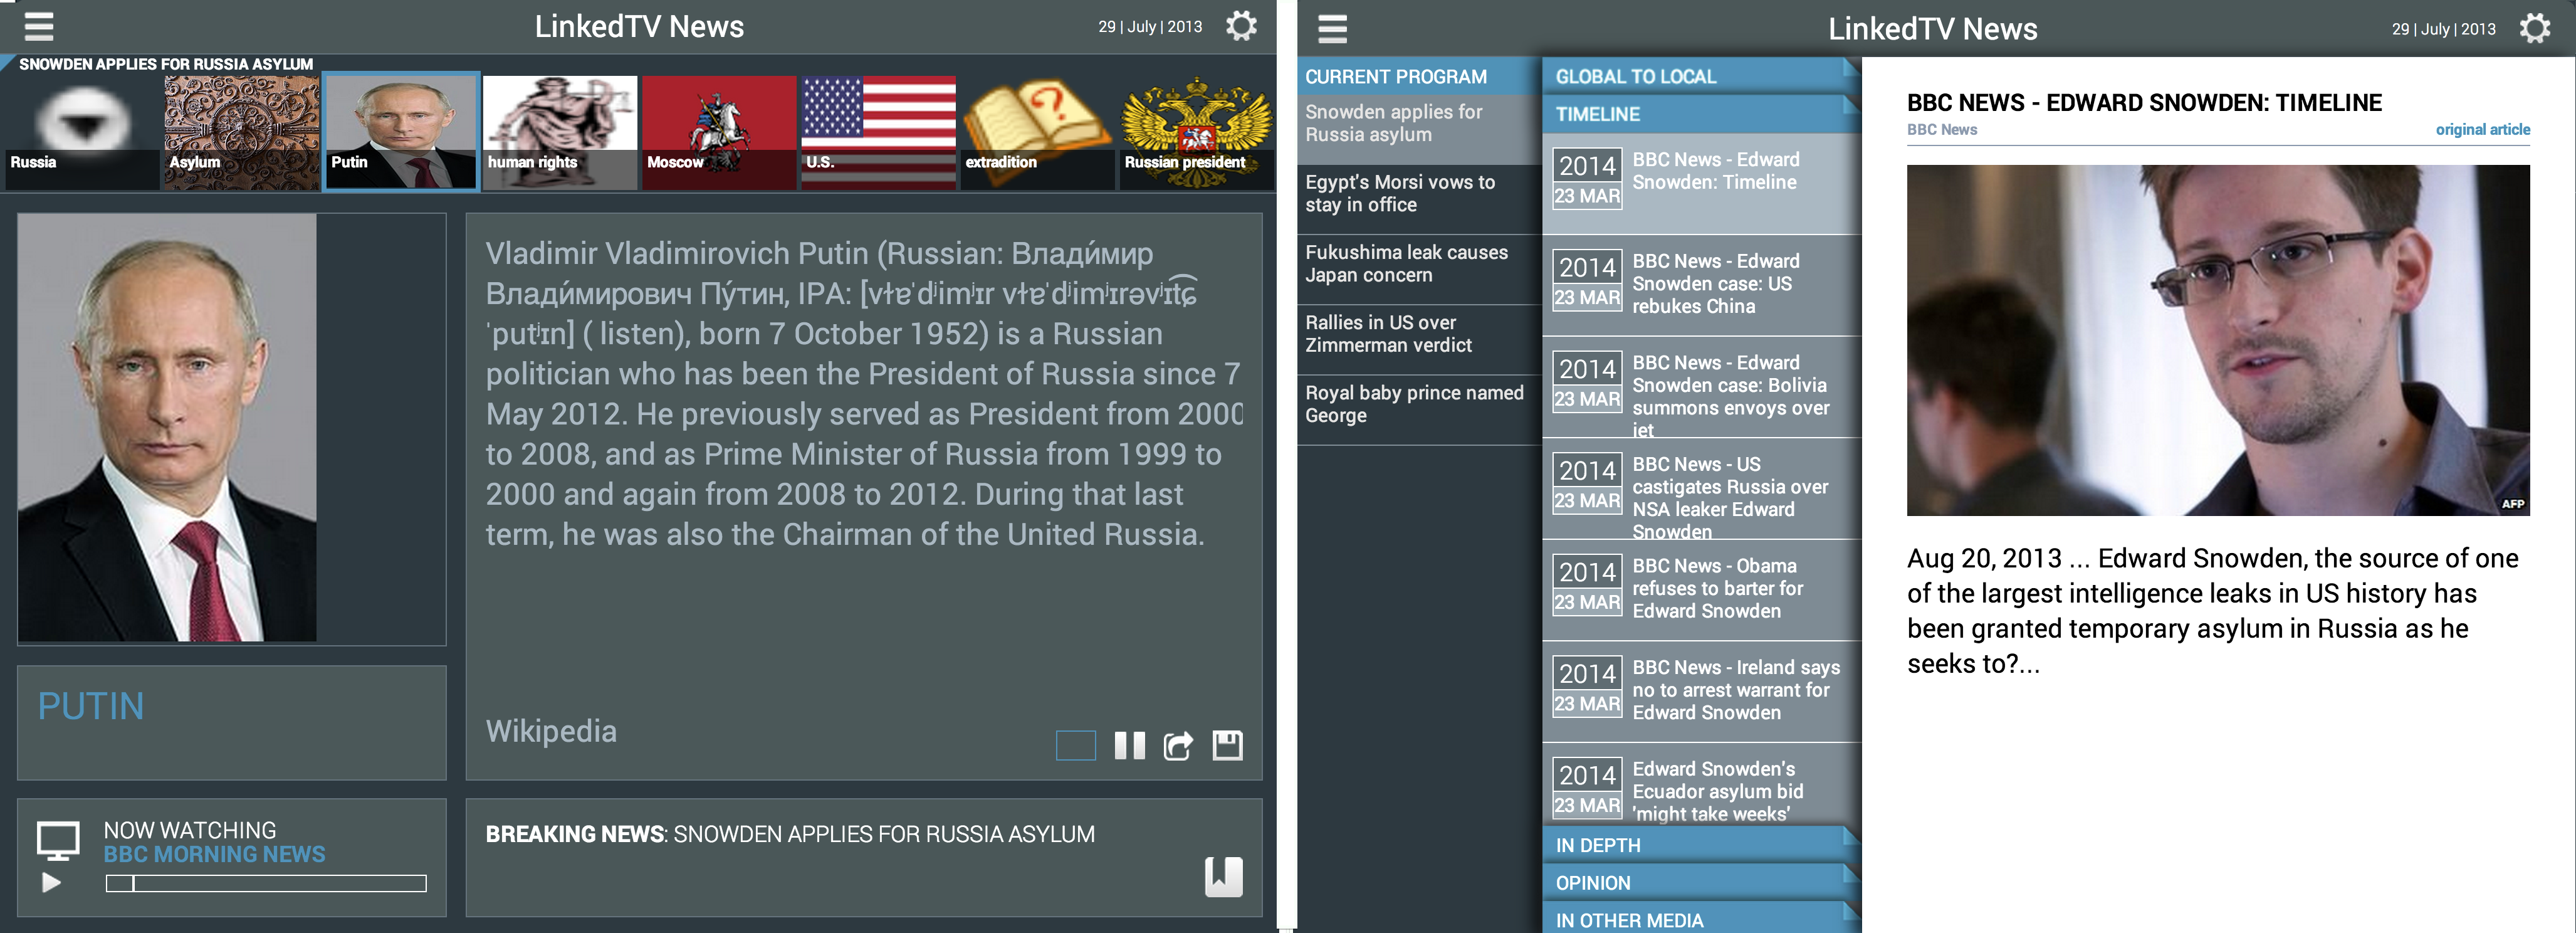
\includegraphics[width=1\textwidth]{figure/DemoScreen}
\caption{Demo screen captures corresponding to the (1) active mode and the (2) passive mode.}
\label{fig:namedEntityExpansion}%\end{figure}
\end{figure}

LinkedTV News is a second screen application for tablets that acts as a companion to viewers when watching news broadcasts. Its main goal is to enrich television newscasts by integrating them with other documents and media via Web knowledge extraction techniques. It is designed to accommodate two viewing modes in terms of interaction: the so called passive and active modes. In the passive mode the application operates as a second screen that is synced with the TV program. This mode supports the user with looking up factual information about the entities that occur in the news. The screenshot on the left side of Figure \ref{fig:namedEntityExpansion} shows the interface of the passive mode. The application shows the content per News item and refreshed when the next item start. The interface contains three parts. At the top it contains a carousel of the entities related to the news item. The middle of the interface show the entity slide with information about the active entity is shown. This information is taken from DBPedia. The bottom part of the interface provides information about the current news item, controls for the video and a button to bookmark the current news item. The passive mode is designed to provide unobtrusive complement to the lean back TV viewing experience. As the entity slides are synced to the content in the video no interaction is required to view the factual content. It is possible to manually select another entity, for example, when information was missed. The design choice for a passive approach with little interaction sets a high demand on the quality of the generated content. 

The bookmark button in the passive mode provide a simple form of interaction by which the user can store a news item. This is in particular useful as a way to let the user switch to the active mode at a later time. In other words, the user can experience the newscast in lean back mode and after the broadcast come back to explore bookmarked items in the active mode. 

The screenshot on the right side of Figure \ref{fig:namedEntityExpansion} shows the interface of the active mode. The left column of the interface shows a list of bookmarked items, the item on Edward Snowden is selected. The middle column shows the five browsing dimenions. The left column shows the article that is currently selected. The browsing dimensions are based on information neends collected from end users. The \textbf{Timeline} dimensions gives the user an overview of past events. The \textbf{Opinion} dimension gives access to articles in which journalists express their opinion about the topic. The dimension \textbf{Other sources} gives different perspectives on the news item as expressed by different news providers. The \textbf{In depth} dimensions allows exploration of more detailed background. The \textbf{Geo-localized information} shows how people in different places in the world respond to the news item on social media. The content for these different dimensions have specific characteristics. To find this content on the Web we need to capture these characteristics in the queries that we submit to the search engine.


%%%  The Passive Mode  %%%
\subsection{Entity extraction and expansion for the Passive Mode}
\label{sec:leanbackmode}

For  the passive mode we need to find the elements of the news, for example, basic information about the location or people involved. The logic that feeds the information displayed in this passive mode is crucial not only because it complements what the user is watching in every moment, but also because it generated the concepts that launch further enrichments in the active mode. To reconstruct the semantic context associated with one particular news video, we perform named-entity recognition over the corresponding subtitles using the NERD framework~\cite{Rizzo2012b}. The output of this phase is a collection of entities annotated using the NERD Ontology\footnote{\fontsize{8pt}{1em}\selectfont \url{http://nerd.eurecom.fr/ontology/nerd-v0.5.n3}}, that comes with a first relevance score obtained from the extractors which have been used. This set includes a list of ranked entities that are explicitly mentioned during the video.

The set of entities obtained from a traditional named entity extraction operation is normally insufficient and incomplete for expressing the context of a news event. Sometimes, some entities spotted over a particular document are not disambiguated because the textual clues surrounding the entity are not precise enough for the name entity extractor, while in other cases, they are simply not mentioned in the transcripts while being relevant for understanding the story. We perform the a process named \emph{entity expansion}, which relies on the idea of retrieving and analyzing additional documents from the Web where the same event is also described. By increasing the size of set of documents to analyse, we increase the completeness of the context and the representativeness of the list of entities, reinforcing relevant entities and finding new ones that are potentially interesting regarding that news item. The entire logic is illustrated in in Figure~\ref{fig:namedEntityExpansion}.

\begin{figure}[t!]
\centering
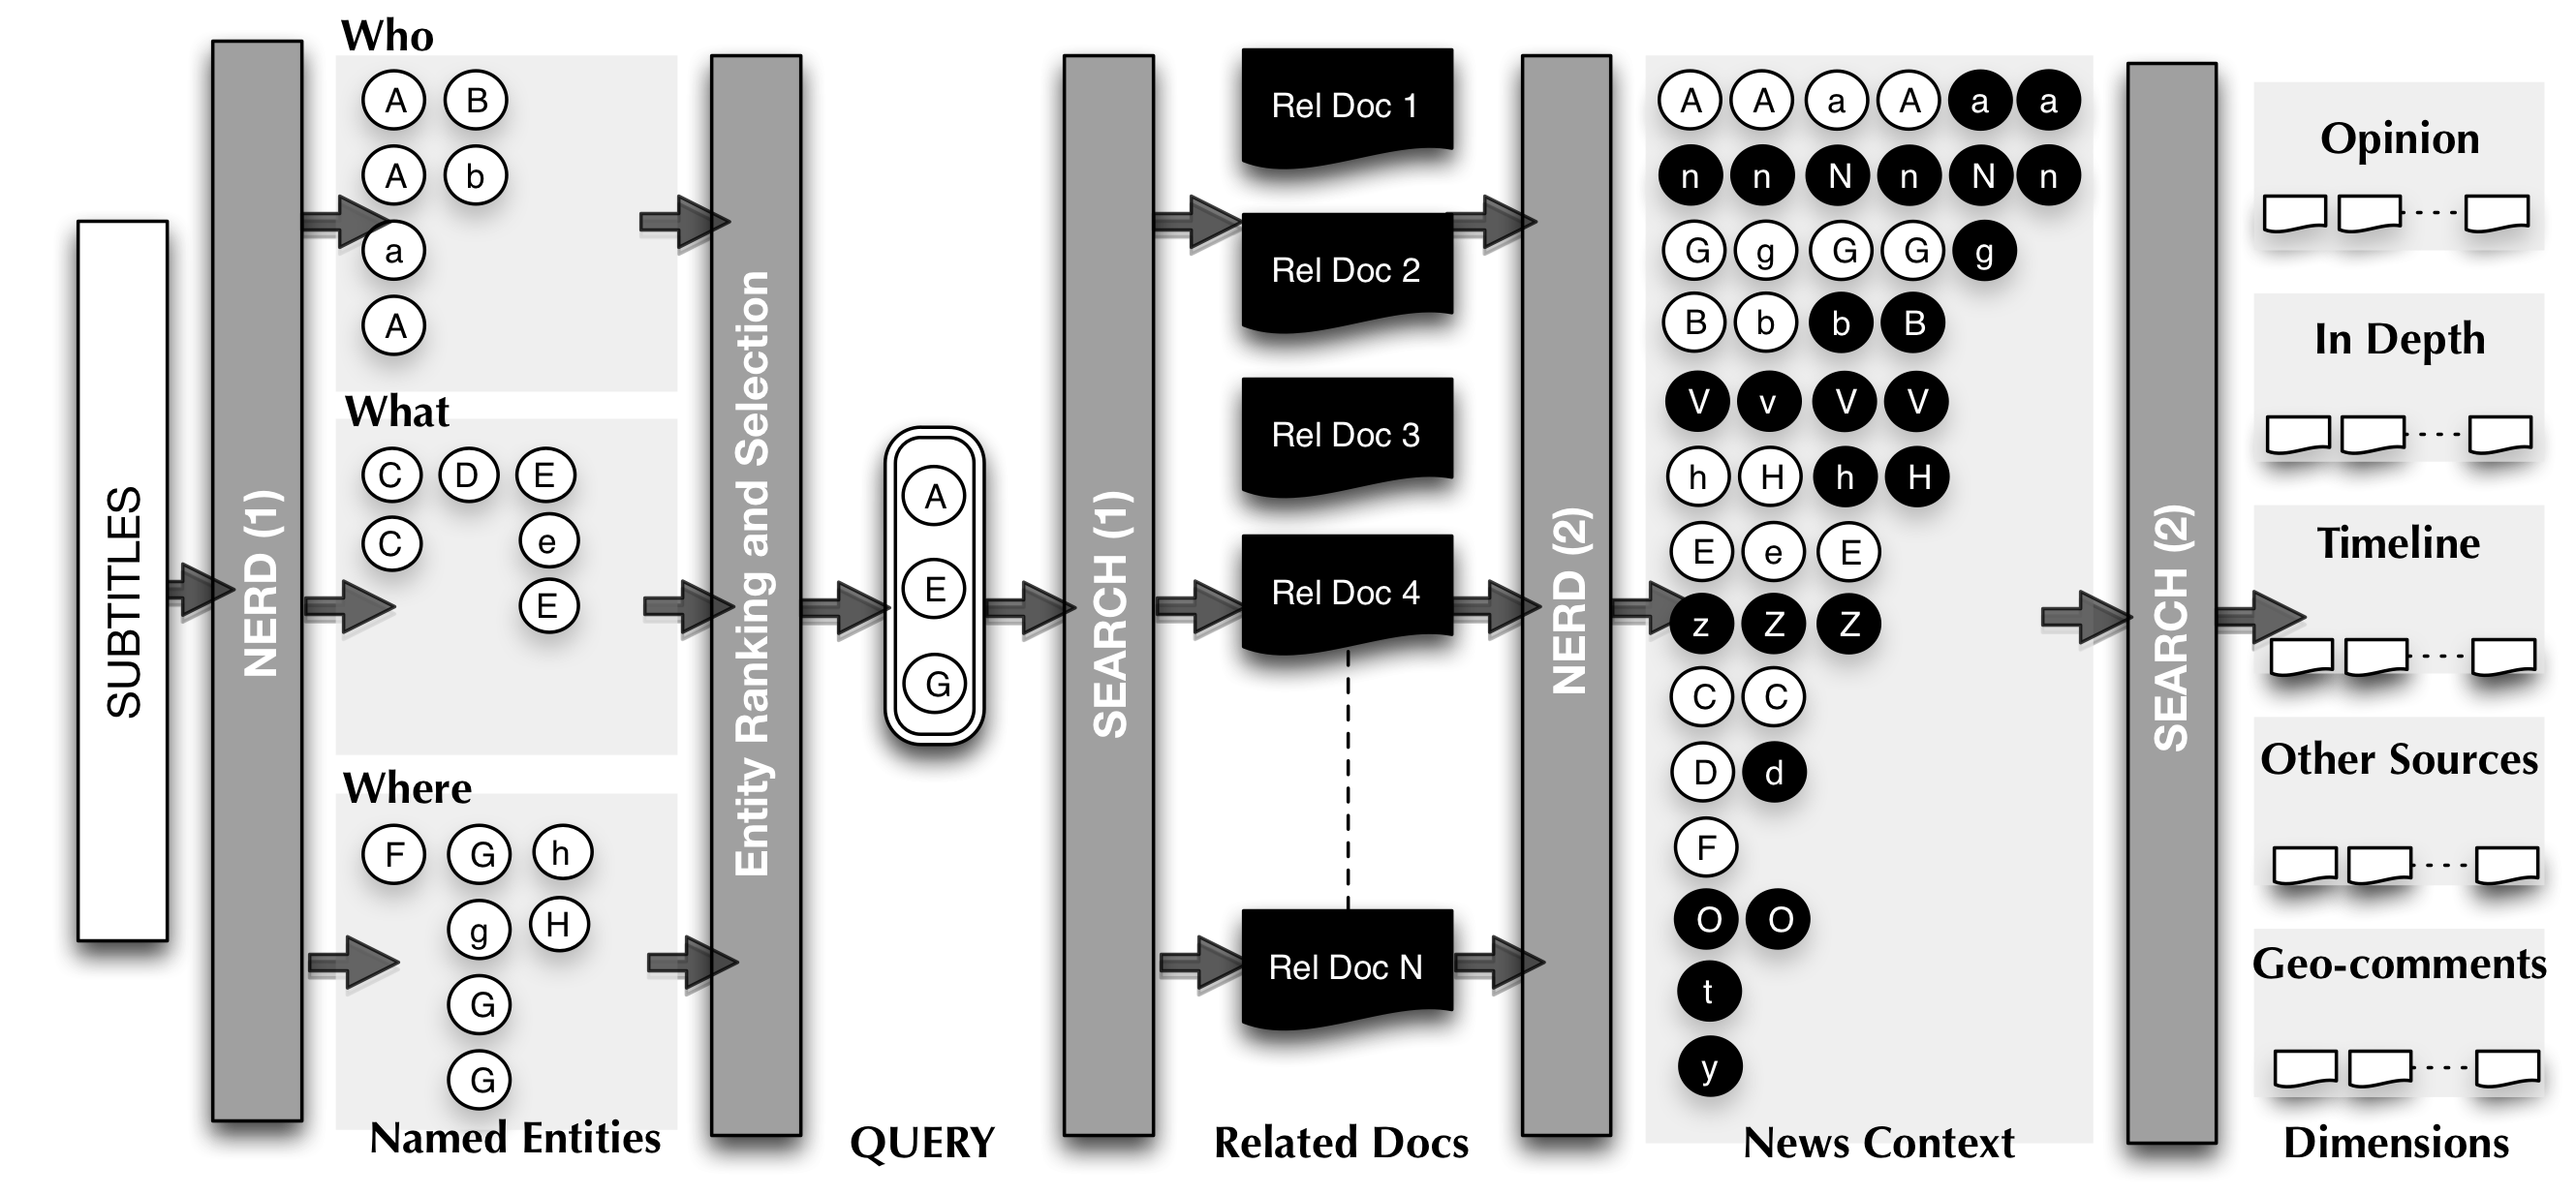
\includegraphics[width=1\textwidth]{figure/ExpansionDiagram}
\caption{Schema of Named Entity Expansion Algorithm.}
\label{fig:namedEntityExpansion}%\end{figure}
\end{figure}

\textbf{Query Generation}The \emph{Five W's} is a popular concept of information gathering in journalistic reporting. It captures the main aspects of a story: who, when, what, where, and why~\cite{LiJia2007}. We try to represent the news item in terms of four of those five W's in order to generate a query that retrieves documents associated to the same event.

In order to achieve this, the original entities are mapped to the NERD Core ontology. From those ten different categories, we generalize to three classes: the Who from \url{nerd:Person} and \url{nerd:Organization}, the Where from \url{nerd:Location}, and the What from the rest of NERD types after discarding \url{nerd:Time} and \url{nerd:Amount}. The When or so-called temporal dimension does not need to be computed since it is considered to be provided by the video publisher. The final query is the result of concatenating the labels of the most relevant entities in the sets Who, What, Where in that particular order, for a given time period dimension $t$.  
This query will be injected into a document search engine (in our case, the Google Search REST API \footnote{\fontsize{8pt}{1em}\selectfont  \url{http://ajax.googleapis.com/ajax/services/search/web?v=1.0}}) where additional descriptions about the news event can be found.

\textbf{Entity Clustering}
In this phase, the additional documents which have just been retrieved are processed and analyzed in order to extend and re-rank the original set of entities and consequently get a better insight about the event. They are again analyzed by the NERD framework in order to extract more named entities. Once finished, we performed a centroid-based clustering operation over the entities retrieved, considering as centroid the entity with the most frequent disambiguation URL's and most repeated label. The output of this phase is a list of clusters containing different instances of the same concept.

\textbf{Entity Ranking}
The final step of the expansion consists of ranking the different named entities obtained so far according to its relative frequency in the transcripts of the event video, relative frequency over the additional document; and average relevance according to the named entity extractors. The final output of the entity expansion operation is a list of entities together with their ranking score and the frequency in both the main video and in the collected documents retrieved from the search engine.

%%%  The Lean-Forward Mode %%%
\subsection{Related content for the Active Mode}
\label{sec:leanforwardmode}
The active mode of the application acts as a hub where the viewers can access extra documents for complementing what is being told in the main news video. A similar logic to the one explained in Section~\ref{sec:leanbackmode} is applied over the main entities coming from the expansion process for building custom queries in Google CSE, but relaxing or emphasizing some particular \emph{W's} and operating over particular lists of Web resources. In contrast to traditional news aggregators that simply gather related documents, the results are organized around five different axes that intent to fulfill the viewer' needs. 

\textbf{Timeline.} Follows the news story throughout time by confectioning an list of ordered documents that includes the main antecedents of the present facts. For getting those document we rely on a query without any prior time constraint, which is created when including the most relevant entity from the Who, Was, Where inside the pattern ''The'' + entity + "case". For our example we have obtained the text "The Edward Snowden case".

\textbf{In other sources.} This section of the interface is dedicated to showing the selected news as it was reported in other newspapers, radio, or TV programs. We launch a query generated from the set of expanded entities by following exactly the same logic used during the entity expansion, over a curated list of resources including mainly Journals and television broadcasters Web sites. In our example the query looks like "Asylum Edward Snowden Russia"

\textbf{Opinion.} This section is devoted to gathering opinions regarding the selected news item from different authors with a certain presupposed knowledge about the matter. The list of documents is obtained by executing the same query generated for dimension ''In other Sources'', but operating over a different list of curated resources that considers only subdomains specialized in opinion documents.

\textbf{Geo-localized information.} This section includes live feeds from Twitter expressing people�s remarks, comments and feelings filtered by subject and geo-location. We use the same query built for the dimension ''In other Sources'', but reducing the temporal dimension $t$ to the last 7 days from the current time in order to see what the people is thinking about the particular news item.

\textbf{In depth.} Includes in depth coverage articles that offer a more extensive view about the seed news item. They documents under this dimension are obtained by combining the most relevant entity from the Who, Was, Where with the keyword "in depth" and removing any temporal restriction and extending the search domain to the entire Web. In our example the textual will be "Edward Snowden in depth";
		
%%%%%%%%%%%%%%%%%%%%%%%
%%%  4. Discussion  %%%
%%%%%%%%%%%%%%%%%%%%%%%

\section{Discussion}
\label{sec:discussion}
The preliminary results indicate that we are able to offer to the viewer a relevant set of entities that expands the initial concepts detected by traditional named entity recognition approaches and covers a wider range of user information needs. Many details not explicitly mentioned in the video but important in the context of the newscasts are now available to the viewer to be consumed, either during he is watching the news in passive mode or when he browses additional insights in the so called active mode.

At the same time those detected concepts are used as powerful triggers for detecting extra knowledge from the Web along 5 main dimensions. Some of those axes are focused on providing the big picture of the news event (\emph{timeline} and \emph{in depth}). Others are intended to help the viewer to corroborate the facts in alternative sources (\emph{in other sources}) and obtain feedback from professionals and journalists (\emph{opinion}). Finally, keeping in mind that TV newscasts viewing is a potentially social activity, one of the dimensions include live feeds from twitter filtered by subject and by geo-location. 

In the future we plan to continue improving the way detected concepts are ranked in relevance and therefore chosen as candidates for answering particular viewer's demands or trigger new enrichments. We also look forward to a more exhaustive evaluation based on viewers' feedback from surveys and open interviews where we can gather more information about which are the viewer's requirements to potentially fulfill the aimed hypervideo experience.

%%%%%%%%%%%%%%%%%%%%%%%%%
%%%  Acknowledgments  %%%
%%%%%%%%%%%%%%%%%%%%%%%%%

\section*{Acknowledgments}
This work was partially supported by the European Union's 7th Framework Programme via the project LinkedTV (GA 287911).

%%%%%%%%%%%%%%%%%%%%%%
%%%  Bibliography  %%%
%%%%%%%%%%%%%%%%%%%%%%
\bibliographystyle{abbrv}
\bibliography{EnrichedTVNews}

\end{document}
